\section{Background}

The interior of a planet affects its surface character. Motions in the mantle are continuously modulating important aspects of the entire planetary system like the volume of its oceans, the composition and pressure of its atmosphere, its surface elasticity, its magnetic field, and its overall climate and habitability \citep{Noack2014, Foley2016, Wordsworth2016, Tosi2017, Wordsworth2018, Shahar2019}. This fact is not always explicit in studies of exoplanets \citep{Shahar2019}, as astrophysics cannot directly constrain geophysical models. Nevertheless, advances brought on by the characterization era of exoplanet science\footnote{i.e., atmospheric spectroscopy} now permit some description of planetary interiors as well, through measurements of a planet's bulk density, the host star chemistry, and the detection of atmospheric species \citep{Santos2017, Dorn2017, Dorn2017a, Dorn2018, Bower2019, Madhusudhan2020}. In this way, exoplanet science is an intrinsically interdisciplinary field, drawing on geophysics and geochemistry to study planets around other stars.

Not only can Earth teach us about exoplanets, but exoplanets can place Earth in an illuminating context. We now know exoplanets are as common as stars, so even basic measurements across a sample have statistical power to complement more detailed studies of the cosmically-unrepresentative solar system. Indeed, other planetary systems are found to be very unlike the one we know: the first detection of an exoplanet revealed this fact with a bafflingly close-in Jupiter-mass world \citep{Mayor1995}. As exoplanet occurrence rate studies reveal \citep{Petigura2013, Foreman-Mackey2014, Dressing2015, Kunimoto2020}, every Sun-like star\footnote{FGK spectral class} in the solar neighbourhood is statistically likely to host at least one planet of mysteriously intermediate mass, between Earth and Neptune---before the detection of exoplanets we had no reason to imagine these existed. 

In the interim, before more detailed observational constraints on massive potentially-rocky planets can be made, there grows a theoretical literature on how geophysical matters scale with mass: internal structure \citep{Valencia2006, Zeng2017}, tidal response \citep{Tobie2019}, outgassing \citep{Kite2009, Noack2017, Dorn2018a}, geodynamos \citep{Gaidos2010}, tectonics \citep{ONeill2007, Korenaga2010}, and so on. Here we are interested in the planet mass-scaling of a particular expression of interior dynamics not typically considered in the exoplanet context: the occurence of topography. Topography is tightly linked to temperatures and mantle flows inside the planet. Therefore the problem is one of understanding a planet's thermal history.

\subsection{Terrestrial planet interiors through time}

%The late stage of planetary accretion leaves a molten and unrecognizable world \citep{Elkins-Tanton2012}. The magma ocean planet crystallizes to rock \footnote{unless the planet's surface is kept too hot such as by proximity to the star, in which case crystallization can take 100 million years, not a few million \citep{Hamano2013}.}, and during cooling, the interior gravititationally differentiates, and volatile species partition between the mantle and the primary crust and atmosphere. These processes set the ``intitial" thermal and chemical state of the solid planet \citep{Tosi2019}. 

The transport of heat through a planet drives much of its dynamics. In the broadest sense, the thermal state of the planet can be described by the ratio of heat production to heat loss; that is, the Urey ratio:
\begin{align}\label{eq:Ur}
{\rm Ur} = \frac{Q_{\rm radiogenic}}{Q_{\rm surface}},
\end{align}
where $Q_{\rm radiogenic}$ and $Q_{\rm surface}$ are the whole planet-integrated fluxes in W of radiogenic heating and surface heat loss, respectively. A young planet can have so much radiogenic heating power that its Ur is much larger than 1. Three things happen with age: the hot core transfers its excess heat into the mantle; its interior abundances of potassium-40, uranium-235, uranium-238 and thorium-232 decline; and the surface loses heat to the atmosphere and eventually to space. This thermal evolution is described via the energy balances,
\begin{align}\label{eq:T_ODE}
\begin{split}
M_m c_{m} \frac{{\rm d}T_m}{{\rm d}t} &= -Q_{\rm u} + Q_{\rm rad} + Q_c, \\
M_c c_{c} \frac{{\rm d}T_c}{{\rm d}t} &= -Q_c,
\end{split}
\end{align}
where $M_m$ is the mantle mass in kg, $c_{m}$ is the mantle specific heat capacity in J kg$^{-1}$ K$^{-1}$, $Q_{\rm rad}$ is the mass-integrated radiogenic heat flux in W, $Q_{u}$ is the magnitude of the surface-integrated heat flux out of the top of the mantle in W (the subscript $u$ denotes the upper boundary layer). The analagous notation with subscript $c$ applies to the core. Although (\ref{eq:T_ODE}) oversimplifies the problem by omitting other heat fluxes like volcanism, it will suffice in capturing the basic behaviour \citep{Jaupart2015}.



\subsection{Parameterized convection models}

The temperature difference between the core-mantle boundary and the lithosphere drives convection, a process that has been modelled to varying degrees of complexity \citep[e.g.,][]{McKenzie1974, Nakagawa2015}. While advanced 3D models are more accurate than lower-dimensional models, running them is computationally expensive. Cheaper 1D parameterized convection models are more reasonable for certain reasearch questions \citep{Sharpe1979, Schubert1980, Davies1980}. When investigating distant planets' topography, where we have little-to-no constraints on the model parameters, computational inexpensiveness allows us to explore a much larger parameter space. Conversely, numerical convection models are better used to predict, for example, the exact shape and distribution of surface topography on Earth or Venus \citep[e.g.,][]{Moresi1995, Vezolainen2004}. 1D parameterized models have previously been applied to planets larger than Earth \citep{Valencia2009, Stamenkovic2012}.

Parameterized models work because most of the interesting behaviour of a convecting cell is controlled by relatively thin thermal boundary layers at the top and bottom of the cell---boundary layers are where the cell's thermal history is effectively determined. Parameterized models will be therefore be valid as long as dynamic processes in the thermal boundary layers occur faster than the planet loses heat \citep{Sharpe1979, Korenaga2008a}. 

As detailed in the appendix to this report, one can write scaling laws for the heat fluxes across the thermal boundary layers. The heat fluxes ultimately depend on the Rayleigh number, Ra. Ra is a nondimensional parameter which quantifies the ``vigour" of convection, and is equal to the ratio of time scales for heat transport by conduction to heat transport by convection:
\begin{equation}\label{eq:Ra}
\mathrm{Ra} = \frac{\tau_{\rm conduction}}{\tau_{\rm convection}}= \frac{\alpha \rho g \Delta T d^3 }{ \kappa \eta(T)},
\end{equation}
where $\alpha$ is thermal expansivity in K$^{-1}$, $\rho$ is density in kg m$^{-3}$, $g$ is surface gravity in m s$^{-2}$, $\Delta T$ is the temperature contrast across the layer in K, $d$ is the thickness of the layer in m, $\kappa$ is the thermal diffusivity in m$^{2}$ s$^{-1}$, and $\eta$ is the dynamic viscosity in Pa s. For a non-isoviscous convecting cell in 2D or 3D, there are many values of viscosity to choose from when defining Ra, so the location this viscosity corresponds to must be specified. Different types of Rayleigh numbers exist, which make different assumptions about what quantity is fixed in the model (the ``thermal" Ra in (\ref{eq:Ra}) fixes $\Delta T$, e.g.), so we must be cautious when comparing between them.

Below a critical Rayleigh number, Ra$_{\rm crit}$, convection is so weak it halts altogether. The value of Ra$_{\rm crit}$ depends on the wavelength of the disturbance that initiates convection, but often a constant value is assumed for a planetary mantle. Ra controls the thermal boundary layer in that the thickness of this layer, $\delta_u$, is approximately the value of $d$ at which convection is inefficient, Ra = Ra$_{\rm crit}$ locally. Therefore $\delta_u \propto {\rm Ra}^{-3}$.

The flux across the upper thermal boundary layer, $q_u$, scales with Ra via $\delta_u$:
\begin{equation}\label{eq:q_Ra}
q_{u} = -k_m \frac{a_{rh} \Delta T_{rh}}{\delta_{u}},
\end{equation}
where $k_m$ is the thermal conductivity in W m$^{-1}$ K$^{-1}$, $\Delta T_{rh}$ is the rheological temperature scale in K, set by the rate of change of viscosity with temperature (see Appendix \ref{sec:methods}), $a_{rh}$ is a constant of order unity, and $q_u$ is in W m$^{-2}$.




\subsection{Regimes of mantle convection}

Stagnant lids appear to be a natural consequence of temperature-dependent convection. Laboratory experiments observing cells of convecting corn syrup or golden syrup show that if the viscosity contrast between the centre and surface is large enough, the upper part of the thermal boundary layer will be dynamically-decoupled from the interior; i.e., not participate in convection at all. These so-called stagnant lids develop in convection cells with large viscosity contrasts \citep{Davaille1993, Giannandrea1993}. Silicate rock does have a strongly temperature-dependent rheology \citep{Karato1993}, and indeed Venus and Mars seem to behave as if they have a stagnant lid. Heat flows through the lid via conduction, while convection occurs only below the lid, where conditions are hotter and more viscous \citep{Morris1984, Christensen1984, Hansen1993, Solomatov1995}. %This fact inspires many questions about whether stagnant lid planets can form ``continents" and other topographic complexities. The character of certain tesserae on Venus imply tectonic origin, questioning whether this world always had a purely stagnant lid \citep{Bindschadler1991, Lenardic1991}. 
This scenario is illustrated in figure \ref{fig:stagnant_lid}.

Stagnant lid behaviour has been reproduced numerically \citep{Solomatov1995, Moresi1995a, Solomatov1996a}. Maps of convective regimes in viscosity contrast-Rayleigh number space can be found in \citet{Solomatov1996a} and more recently in \citet{Huttig2011} and \citet{Miyagoshi2015}, with stagnant lids favouring higher Rayleigh numbers \textgreater~$10^{6}$--10$^{7}$ and viscosity contrasts \textgreater~$10^4$ between the interior mantle and the surface.

We consider a stagnant lid regime under the premise that it represents a ``default" rocky planet \citep{ORourke2012}. In our own solar system, rocky planets are more frequently found in a stagnant lid regime than in a plate tectonic regime. With the assumption of a stagnant lid we avoid some unknown complexities that mobile plates introduce. Namely, plate margin-dominated heat loss on Earth works differently \citep[and more efficiently---stagnant lid planets will run hotter for the same rheology and surface heat flow;][]{Stevenson2003} than in a stagnant lid regime, where heat loss is simply determined by boundary layer scaling laws like those we have discussed.


\begin{figure}

  \centering
  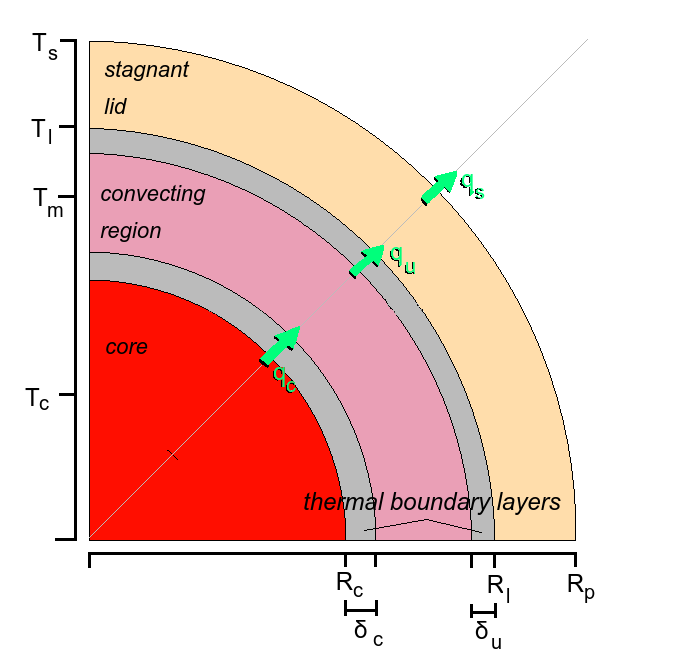
\includegraphics[width=0.5\linewidth]{stagnantlid}

\caption{Structural model of a stagnant lid planet, not to scale. $R_p$ is the radius of the planet, $R_l$ is the radius at the base of the lid, $R_c$ is the radius of the core, $T_s$ is the surface temperature, $T_l$ is the temperature at $R_l$, $T_m$ is the isothermal convecting cell temperature, $T_c$ is the isothermal core temperature, and $\delta_u$ and $\delta_c$ are the upper and lower thermal boundary layer thicknesses respectively. The boundary layer heat fluxes $q_c$ and $q_u$ and the surface heat flux $q_s$ are defined in equations (\ref{eq:q_Ra}) and (\ref{eq:q_s}), respectively}. 
\label{fig:stagnant_lid}
\end{figure}







\subsection{Stress and topography}

Earth is hypsometrically bimodal: continents and oceans form separate peaks in the hypsometric curve. This is a complexity not seen on Mercury, Venus, the Moon, or Titan \citep{Keller2009, Lorenz2011}.\footnote{Mars has dichotomous crustal thickness split between its north and south hemispheres. This produces bimodality for different reasons than Earth, a further complexity.} Earth's topography is much more convoluted than anything a parameterized convection model could predict. Topography on stagnant lid planets, however, is more tenable to modelling.


\subsubsection{Mechanisms of topographic support}\label{sec:top_mechs}


To predict topography, we need to look at the forces balancing topographic loads. The first two mechanisms we discuss are not the focus of this document, but are nevertheless associated with the most dramatic topography on planets:
\begin{enumerate}
\item \emph{Elastic flexure} of a shell supports loads by way of elastic stresses that develop in the lithosphere;
\item \emph{Airy or Pratt isostasy} occurs when high mountains made of low-density crust are underlain by either deep roots of the same low density (Airy), or by roots of the same thickness as the surrounding plain but of lower density (Pratt).
\end{enumerate}
Whether a load is supported by (1) or (2) is set by the ratio of the width of the load to a flexural parameter, which depends on the lithosphere's elastic properties.\footnote{$\alpha_{\rm flex} = \left[\frac{1}{3(1 - \nu^2)}\frac{Ed_e^3}{\rho_m g}\right]^{1/4}$, where $d_e$ is the lithosphere thickness, $\rho_m$ is the underlying mantle density, $\nu$ is Poisson's ratio, and $E$ is Young's modulus.}
%\begin{equation}
%\alpha_{\rm flex} = \left[\frac{1}{3(1 - \nu^2)}\frac{Ed_e^3}{\rho_m g}\right]^{1/4},
%\end{equation}
%where $d_e$ is the lithosphere thickness, $\rho_m$ is the underlying mantle density, $\nu$ is Poisson's ratio, and $E$ is Young's modulus. 
If the width of a load is smaller than the flexural parameter, elastic stress in the lithosphere will support the load. If the width is much larger, buoyancy forces will support it. Hence flexure is associated with short-wavelength topography and isostasy is associated with long-wavelength topography. 

The last support mechanism is borne by convection in the interior. Historically the term has always not referred to the same phenomena, so it is helpful to break down \emph{dynamic topography} further \citep{Orth2011, Molnar2015} into:
\begin{enumerate}
\setcounter{enumi}{2}
\item \emph{Flow-induced tractions} on the base of the lithosphere. These tractions are exerted by the deformation of density boundaries within the viscously-flowing material below the thermal boundary layer.
\item \emph{Thermal isostasy,} variations in the thickness and thermal structure of the upper boundary layer \citep{Fowler1985}. On Earth this can be split into lithospheric and aesthenospheric components, but for planets without plates, this collapses to just variations in the viscous lid \citep[see][]{Orth2011}. This is unlike Airy and Pratt isostasy in that the density contrasts are thermal rather than compositional. Thermal isostasy provides the majority of ``dynamic topography."\footnote{Analytically we expect component 4 to dominate component 3 for an idealized sine-curve temperature perturbation at the surface, regardless of the wavelength of that perturbation \citep{McKenzie1977}. It can be shown that the gravity anomaly $\Delta g_1(x)$ considering no density contrast in the lithosphere, just the lithosphere's deflection upwards, is $\Delta g_1(x) = 2\pi G \Delta \rho \Delta h(x)$, where $G$ is the gravitational constant and $\Delta h$ is the height of topography. The gravity anomaly $\Delta g_2(x)$ associated with the flow-induced density contrasts alone is $\Delta g_2(x) = 2\pi/3 \; G\rho\Delta h_2(x)$. For a given gravity anomaly, $\Delta h_1 > \Delta h_2/3$.}
\end{enumerate}
Together, components 3 and 4 make the ``full dynamic topography." In a given model, teasing out the distinction between components 3 and 4 can present a problem when comparing between models, as we will see in section \ref{sec:dyn_top_ss}. 
%The distinction between components 3 and 4 matters, not necessarily because different parties disagree with their competing importance (on Earth), but because ``dynamic topography" does not consistently refer to either or both components. %In some circumstances, the two mechanisms can even produce identical signals \citep{Molnar2015}. 



%It can be shown that the topography associated with (3) is about a third of the topography associated with (4) \citep{McKenzie1968, McKenzie1977, Molnar2015}. 


\subsubsection{Dynamic topography forward models}\label{sec:dyn_top_forward}

%\citet{McKenzie1968, 1977} derives analytic half-space equations for $\Delta h$ as a function of a harmonic temperature perturbation $T(x) = T_0 \cos(2\pi x/\lambda)$, associated with both static and dynamic density contrasts, In both cases the solution for $\Delta h(x)$ is propotional to $\alpha T_0 \lambda / (2\pi) \cos(2\pi x/\lambda)$, with the static scenario a factor of \nicefrac{4}{3} higher because it does not have to overcome resistance to flow from an additional vertical shear stress term (Stokes equation). 

Numerical models can calculate the amplitude of the dynamic component of topography, $\Delta h$, by solving the equations of motion and the heat transport equation for a convecting cell, and obtaining the velocity and temperature fields. The total stress in the vertical direction, $\tau_{zz}$, can then be calculated at the surface of the cell. Total vertical stress is given by 
\begin{equation}\label{eq:tau_zz}
\tau_{zz} = 2\eta \; \frac{\partial u_z}{\partial z} - p_1,
\end{equation}
where $\partial u_z / \partial z$ is the vertical velocity in m s$^{-1}$ and $p_1$ is the pressure pressure perturbation from thermal convection in Pa \citep{Parsons1983}. The first term in (\ref{eq:tau_zz}) is the viscous stress. The hydrostatic pressure $p_0$ of a topographic load balances this stress, $p_0 = \rho g \Delta h = \tau_{zz}$, where $\Delta h$ is in m. Combining this and (\ref{eq:tau_zz}) with self-consistent pressure and temperature profiles inherently includes both dynamic topography components, producing the full dynamic topography,
\begin{equation}\label{eq:h_stress}
\Delta h = \frac{\tau_{zz}}{\rho g}.
\end{equation} 

To separate the thermal and flow-induced components of (\ref{eq:tau_zz}), expressions for the maximum topography due solely to thinning of the lithosphere can be derived: 
\begin{equation}\label{eq:h_th}
\Delta h \sim 0.5\alpha (T_i - T_s) z_{l, 0},
\end{equation}
where $T_s$ is the surface temperature in K, $T_i$ is the temperature below the lithosphere in K at the point of interest, and $z_{l, 0}$ is the average thickness of the lithosphere in m \citep{Kucinskas1994, Orth2011}. Although this thermal thinning component may explain most of the full dynamic topography on stagnant lid planets, using (\ref{eq:h_th}) to approximate dynamic topography \citep[the ``isostatic stagnant lid approximation";][]{Orth2011} requires knowledge of the lateral variations of temperatures under the lithosphere, which is not possible with 1D models.


In principle, one can obtain $\tau_{zz}$ in (\ref{eq:tau_zz}--\ref{eq:h_stress}) from parameterized convection, since the upper thermal boundary layer contributes most of the depth-integrated stress \citep{Parsons1983, Solomatov1995}. The parameterized stress is given by
\begin{equation}\label{eq:tau_param}
\tau_{zz} = C_1 \alpha_m \Delta T_{rh} \delta_u.
\end{equation}
\citet{Reese2005} give proportionality constant $C_1 = 2$ for the shear stress at the lid generated by sinking plumes, based on fits to a numerical convection model with spherical geometry and temperature-dependent viscosity. We note that it is the normal component of stress, not the shear stress, that balances $\rho g \Delta h$. However, no other scaling is available to our knowledge, so we adopt this value as a preliminary measure. We treat $\tau_{zz}$ as the planetary root-mean-square (RMS) value for convective stress, producing the RMS dynamic topography, $\Delta h_{\rm RMS}$. 

According to (\ref{eq:tau_param}), we expect $\Delta h_{\rm RMS}$ to scale with the RMS thermal boundary layer thickness, which scales with Ra as $\delta_u \propto {\rm Ra}^{-3}$. The strength of this scaling would be affected by other modelling decisions, such as the rheology law and the amount of internal heating compared to basal heating \citep{McKenzie1977}. Under particular model assumptions, scalings of $\Delta h$ with Ra can be found in the existing literature.

For the first scaling, we combine (\ref{eq:h_stress}) and (\ref{eq:tau_param}) in terms of Ra via (\ref{eq:d_u}):
\begin{equation}\label{eq:dyn_top_stress}
\Delta h_{\rm RMS} \sim \alpha_m d \Delta T_{rh} \left(\frac{\rm Ra}{\rm Ra_{\rm crit}}\right)^{-\frac{1}{3}}.
\end{equation}
(\ref{eq:dyn_top_stress}) is equivalent to equation (34) in \citet{Parsons1983}, which is a boundary-layer-based approximation of their equation (33),
\begin{equation}\label{eq:PD83_0}
\Delta h = C_2 \frac{\eta_m \kappa_m}{\rho_m g d^2} \left({\rm Ra}_F\right)^n,
\end{equation}
where Ra$_F$ is the Rayleigh number based on surface heat flux,\footnote{Ra$_F = (\rho g \alpha d^4 q_u)/(k \kappa \eta)$} $n = 0.5$ \citep{McKenzie1977}, and $C_2 = 5.4$ to match the predictions of RMS dynamic topography in \citet{Lees2019} using a 3D isoviscous basal-heating convection model. Although it can be misleading to convert between Ra and Ra$_F$ as the model assumptions are fundamentally different, we can approximate (\ref{eq:PD83_0}) as a function of Ra with $n = 0.5$, using Ra$^{4/3} = \Delta T_m / \Delta T_{rh} {\rm Ra}_{\rm crit}^{1/3} {\rm Ra}_F$. This gives us the second scaling,
\begin{equation}\label{eq:PD83}
\Delta h_{\rm RMS} \sim \alpha_m d \left[\frac{a_{rh} \Delta T_{rh} \Delta T_m}{{\rm Ra}_{\rm crit}^{\frac{1}{3}}}\right]^{\frac{1}{2}} {\rm Ra}^{-\frac{1}{3}},
\end{equation}
where $a_{rh}$ is the rheological temperature scale prefactor \citep[equal to 2.44;][]{Thiriet2019}, and $\Delta T_m$ is the temperature difference across the convecting region in K. As expected, the exponent on Ra in (\ref{eq:PD83}) is equal to the exponent on Ra in (\ref{eq:dyn_top_stress}). The positive value of $n$ in (\ref{eq:PD83_0}) implies that topography increases with Ra$_F$ in this scaling---this is misleading because $\eta$ is outside of the exponential term.

The third scaling is a direct log-log fit by \citep{Kiefer1992} to the \emph{peak} value of $\Delta h$ over a mantle plume versus Ra, using a 2D cylindrical isoviscous numerical convection model applied to Venus:
\begin{equation}\label{eq:KH92}
0.7 \Delta h = 66 {\rm Ra}^{-0.121},
\end{equation}
where the factor of 0.7 = $(\rho_m - \rho_{\rm ocean} / \rho_m$ scales their water-loaded model to subaerial topography. We further scale this $\Delta h$ by 0.707 (the RMS value of a sine wave) to approximate $\Delta h_{\rm RMS}$.

 



























\begin{landscape}
\thispagestyle{empty}
%\begin{table}

\footnotesize


\begin{longtable}{ @{} p{4cm} r r p{2cm} p{2cm} r p{1.5cm} p{3.2cm} p{3.1cm} @{} } 
\caption{Predictions from numerical convection of dynamic topgraphies on Venus, with important model parameters noted. Internal heating is calculated as $(q_s - q_b)/q_s$, where $q_s$ and $q_b$ are the surface and basal heat fluxes in W m$^{-2}$ respectively. Reported values of the Rayleigh number are distringuished between that defined with a fixed temperature contrast, Ra (\ref{eq:Ra}), and that defined with a fixed basal heat flux, Ra$_B$. \;\;  *Calculated from the spherical harmonic power spectrum using $\Sigma_l [S(l)/(2l + 1)]^{1/2}$.} \label{tab:dyn_topo_obvs}\\



\toprule
\; & \multicolumn{2}{c}{\textsc{Dynamic topography} (km)} \\
\cline{2-3} \\
\textsc{Reference} & \textsc{Peak} & \textsc{RMS} & \textsc{Location} & \textsc{Viscosity} & Ra & \textsc{Internal heating} & \textsc{Model type} & \textsc{Dominant component}\\
\midrule 

\citet{Kiefer1991} & \makecell[tr]{7.5 \\ 5.2 \\ 3.6} & n/a  & multiple Regiones &  $f(z)$ & \makecell[tr]{Ra = $10^5$ \\ Ra = $10^6$ \\ Ra = $10^7$} & 0\% & Cylindrical plume & Viscous stress  \\
% after  \citep{Hager1985}


%\citet{Kiefer1992} &  7.5  & n/a & Global & Ra = $10^6$ & $\eta_m$ constant with high-$\eta$ stagnant lid & Numerical cylindrical plume & (3) & for $D_{\rm lid}$ = 130 km; gives scaling laws with Ra, assumes no internal heating (bottom of page 203). h from figure 9 constant visc \\$f(T)$


\citet{Moresi1995} & \makecell[tr]{5.8 \\ 3.8 \\ 5.1} & n/a & Atla Regio  &  \makecell[tl]{$f(T)$ \\ $f(T,z)$ \\ $f(T,z)$} & \makecell[tr]{Ra$_B$ = 2.4 $\times 10^6$ \\ Ra$_B$ = 1.3 $\times 10^6$ \\ Ra$_B$ = 1.0 $\times 10^6$} & 0\% & Axisymmetric convection & Thermal isostasy  \\
% Scaling: $\eta_0 \kappa / (d^2 \Delta\rho g)$ with $\eta_0$ from basal heating Ra, can't extrap to higher $\Delta\eta$ with linearized viscosity law. concerned with predicting admittance
 %

\citet{Nimmo1996} &  \makecell[tr]{1.16 \\ 1.47 \\ 2.85}  &  n/a  & Global & constant & \makecell[tr]{Ra$_B$ = 1.6 $\times 10^7$ \\  Ra$_B$ = 7.9 $\times 10^6$\\ Ra$_B$ = 4.0 $\times 10^6$ } & 0\% & Axisymmetric plume & Viscous stress \\



\citet{Solomatov1996a} & \makecell[tl]{$\sim$4 \\ $\sim$2} & n/a  & \makecell[cl]{Beta Regio \\ Average} & $f(T)$  & Ra = $3 \times 10^7$  & 0\% & Cartesian convection & Thermal isostasy  \\
%Beta Regio (avg) scaled so admittance is 30 (15) m/km, fixed $d_m$ = 1600 km 



\citet{Kiefer1998} &  5.4--10.9 & 1.6--2.7  & Global & constant & Ra = $10^6$ & 73 \% & Hemispherical axisymmetric convection & Thermal isostasy \\
% Scaling: $(\rho_m \alpha \Delta T R_p) / (\rho_m - \rho_s)$  internal heating Ra $10^7$

\citet{Vezolainen2003} & 3.5--6 & n/a & Beta Regio & $f(T)$  & Ra = $3 \times 10^7$ & 0\% & 2D Cartesian plume & Thermal isostasy  \\
%  fixed $\Delta T_m$ = 1100 K

\citet{Vezolainen2004} & 5.7 & n/a & Beta Regio & $f(T)$  & Ra = $3 \times 10^7$ & 0\% & 3D Cartesian plume & Thermal isostasy  \\
%  fixed $\Delta T_m$ = 1100 K



%\citet{Orth2011} & 2.2 nondim & n/a  & Global &  Frank-Kamenetskii & Ra$_i$ = 10$^7$ & 0\% & 3D spherical shell & Thermal isostasy \\



\citet{Golle2012} & 3.3 & 2.7*  & Global & $f(z)$ & Ra$_b = 3.8\times 10^8$ & 0\% & Viscoelastic deformation coupled with thermal convection &  Not enough information \\



\citet{Benesova2012} &  3.25 & n/a   & Alta Regio  & $f(z)$ & Ra = $2.8 \times 10^6$ & \textgreater 50\% & 3D spherical convection & Viscous stress \\
% specifically say no thermal isostasy, although Orth thesis says they do implicitly?



\citet{Huang2013} & 2\textendash 3 & 0.75 & Global & $f(T,z)$ & Ra = $1.8\times 10^7$ & 75\% & 3D spherical convection & Viscous stress \\
% goal is to simultaneously match number of plumes and GTR observations. semi-amplitude by eye from maps.  say case 15 is best fit to obvs. Ra fixed, using avg viscosity $2\times 10^{21}$ Pa s

\citet{Yang2016} & n/a & 0.27* & Global & $f(T,z)$ &  Ra = $7.3\times 10^6$ & 80\% & 3D spherical convection & Viscous stress \\
% they say "The gravity anomaly is the summation of that caused by the dynamic topography and by the density heterogeneity itself." and "the topography of volcanic rises is mainly due to dynamic uplift"


\bottomrule


\end{longtable}
%\end{table}
\end{landscape}


\begin{table}
\centering
\caption{Parameters used in this study. \label{tab:params}}
\footnotesize
\begin{tabular}{@{} c l r l p{4cm} @{}}
%\multicolumn{5}{l}{\textbf{Constant values for all planets}} \\
\toprule
Symbol & Description & Value & Units & Ref. \\
\midrule
\multicolumn{5}{c}{\textbf{Constant bulk properties}} \\
$\rho_c$ & Core density & 7200 & kg m$^{-3}$ &  \citet{Thiriet2019}  \\
$c_c$ & Core specific heat at constant volume & 840 & J kg$^{-1}$ K$^{-1}$  & \citet{Thiriet2019}  \\
$k_m$ & Mantle thermal conductivity & 4 & W m$^{-1}$ K$^{-1}$  & \citet{Thiriet2019}  \\
$\alpha_m$ & Thermal expansivity &  $2.5 \times 10^{-5}$ & K$^{-1}$  & \citet{Thiriet2019}  \\
$\kappa_m$ & Thermal diffusivity &  $1 \times 10^{-6}$ & m$^2$ s$^{-1}$  & \citet{Thiriet2019}  \\
$X_{\rm K}$ & Initial K abundance &  305 & wt ppm  & \citet{Jaupart2015} \\
$X_{\rm U}$ & Initial U abundance &  $16 \times 10^{-3}$ & wt ppm  & \citet{Jaupart2015} \\
$X_{\rm Th}$ & Initial Th abundance &  $56 \times 10^{-3}$ & wt ppm  & \citet{Jaupart2015} \\
$H_{4.5}$ & Radiogenic heating rate at 4.5 Gyr & $4.6\times 10^{-12}$ & W kg$^{-1}$ & \citet{Jaupart2015} \\
Ra$_{\rm crit}$ & Critical Rayleigh number & 450 &  & \citet{Thiriet2019}  \\
$E_a$ & Viscosity activation energy & 300 & kJ mol$^{-1}$ & \citet{Karato1993} \\
$A_{rh}$ & Viscosity preexponential factor & 8.7 $\times 10^{15}$ & & \citet{Karato1993} \\
$h_{rh}$ & Grain size & 2.07 & mm & \\
$B$ & Burgers vector & 0.5 & nm & \citet{Karato1993} \\
$m$ & Grain size exponent & 2.5 & & \citet{Karato1993} \\
$\mu$ & Shear modulus & 80 & GPa & \citet{Karato1993} \\
CMF & Core mass fraction & 0.3 & & \\
$L_*$ & Stellar luminosity & 1 & $L_{\rm Sun}$ &  \\
Al & Planetary geometric albedo & 0 & &  \\

\midrule
\multicolumn{5}{c}{\textbf{Solar system models}} \\
$M_p$ & Planet mass &  \makecell[tr]{\textbf{Mars:} 0.11 \\ \textbf{Venus:} 0.82} & \makecell[tl]{$M_\oplus$ \\ $M_\oplus$ } &  \\
$R_p$ & Planet radius &  \makecell[tr]{\textbf{Mars:} 3390 \\ \textbf{Venus:} 6050} & \makecell[tl]{km \\ km } &  \\
$R_c$ & Core radius &  \makecell[tr]{\textbf{Mars:} 1700 \\ \textbf{Venus:} 3330} & \makecell[tl]{km \\ km } &  \makecell[tl]{\citet{Thiriet2019} \\ \citet{Huang2013}} \\
$\rho_m$ & Mantle density & \makecell[tr]{\textbf{Mars:} 3500 \\ \textbf{Venus:} 3300} & \makecell[tl]{kg m$^{-3}$ \\ kg m$^{-3}$} &   \makecell[tl]{\citet{Thiriet2019} \\ \citet{Nimmo1996}} \\
$c_m$ & Mantle specific heat (p or v?) & \makecell[tr]{\textbf{Mars:} 1142 \\ \textbf{Venus:} 1200} & \makecell[tl]{J kg$^{-1}$ K$^{-1}$ \\ J kg$^{-1}$ K$^{-1}$}  & \makecell[tl]{\citet{Thiriet2019} \\  \citet{Nimmo1996}}  \\
$T_s$ & Surface temperature & \makecell[tr]{\textbf{Mars:} 250 \\ \textbf{Venus:} 730} & \makecell[tl]{K \\ K} \\

\midrule
\multicolumn{5}{c}{\textbf{Initial conditions}} \\
$T_{m,0}$ & Initial mantle temperature & 1750 & K & \citet{Thiriet2019}\\
$T_{c,0}$ & Initial core temperature & 2250 & K & \citet{Thiriet2019} \\
$D_{l,0}$ & Initial lid thickness & 300 & km & \citet{Thiriet2019}\\
\bottomrule
\end{tabular}
\end{table}



\subsubsection{Dynamic topography in the solar system}\label{sec:dyn_top_ss}

We aim to quantify the contribution of dynamic topography to total topography for solar system bodies so we can test our theoretical model of dynamic topography, but this is not so easy because the dynamic component of topography can be tricky to parse from observed topographic heights. Out of the terrestrial planets and moons, we have focused on Venus because of the general agreement in the literature that for certain highland locations, its observed topography can be represented by the full dynamic topography (\ref{eq:tau_zz}). 

%Here we give a short overview of attempts to model dynamic topography on stagnant lid planets. One can estimate the apparent depth of isostatic compensation using satellite measurements of the absolute topography and gravity or geoid anomaly. Larger values of the geoid with respect to the topography imply deeper isostatic compensation depths. Variations in the height of the geoid reflect distortions in density boundaries. %Inferences of dynamic topography are therefore quite sensitive to the assumed viscosity structure \citep{Karato2008a}.

%Another complementary approach \citep[e.g.,][]{Smrekar1991, Kucinskas1994} is to assume Airy isostasy and predict the gravity anomaly resulting from a loading at some depth. Comparing this to observed topography produces a guess of the isostatic compensation depth. If these predictions are far from reality, one concludes that isostasy does not provide all the support. We focus on the convection-based approach, which is more applicable to our needs. Nevertheless, the fact that such models have not reproduced the observed relationships between gravity and topography \citep{Kiefer1986} has been criticized \citep{Orth2011} in its conclusion that isostasy is irrelevant for certain features on Venus, and that Venusian ``dynamic" topography is purely tractional. This is because the arguments against isostasy are necessarily based on assumptions about how thick the realistic crust could be, which is not well constrained.

\vspace{0.5cm}

\textit{\color{teal1} Venus.} Although Venus is hypsometrically unimodal, unlike Earth and Mars, satellite altimetry reveals vast lowland plains dotted with areas of higher elevation. These elevated regions can be grouped into five older highland plateaux, steep-sided 2 km-high landmasses, and nine younger, dome-like volcanic rises \citep{Phillips1998}. Several of the volcanic rise features have been labelled active hotspots \citep{Kiefer1991, Smrekar1991, Grimm1992, Smrekar1994, Stofan1995, Smrekar2010}. The arrival of the Magellan spacecraft into Venus orbit in the 1990s brought gravity and topography measurements, and an influx of research followed, attempting to diagnose how its topography is supported. 

Based on the inferred relationships between its gravity or geoid and its topography, Venus' volcanic rises seem consistent with dynamic topography, while the highland plateaux are likely supported by Airy isostasy \citep{Kiefer1986, Grimm1991, Kiefer1991, Smrekar1994, McKenzie1994, Kucinskas1994, Smrekar1996, Nimmo1996, Simons1997, Pauer2006, James2013, Yang2016}. The dichotomy is not precise, and some regions are not fit by either a purely dynamic and a purely isostatic model. 

Under the paradigm that volcanic rises are dynamically-supported, modellers have been attempting to reproduce observed profiles of individual topographic features on Venus using numerical models of mantle plumes \citep{Kiefer1991, Kiefer1992, Moresi1995, Nimmo1996, Smrekar1996, Kiefer1998}. These numerical modelling efforts are summarized in Table \ref{tab:dyn_topo_obvs}. Table \ref{tab:dyn_topo_obvs} also lists predictions of Venus' topographic spectra from 2D and 3D convection simulations \citep{Golle2012, Benesova2012, Huang2013, Yang2016}. We are concerned with the output of convection models, not the absolute value of Venus' topography, since we are still not agreed on the actual dynamic component of its topography globally.


Advances in numerical modelling, such as including strongly-temperature-dependent viscosity (as expected for terrestrial planets) in at least two dimensions, have bestowed the current understanding that spatial variations in lithosphere thickness under thermal isostasy explain essentially all of Venus' full dynamic topography \citep{Kucinskas1994, Moore1995, Moore1997, Solomatov1996a, Orth2011}. That is, models approximating dynamic topography with only the thermal isostasy component have reproduced the heights of observed peaks on Venus. The requisite lateral variations in lithosphere thickness cannot be reproduced if viscosity is constant or depth-dependent. Nevertheless, we focus on studies that do include the tractional component of dynamic topography because the thermal isostasy approximation does not apply to 1D models.

%\begin{itemize}
%\item refer to definition crisis a bit more, maybe refer reader to column in Table \ref{tab:dyn_topo_obvs} where you sort these where possible
%\item do Parsons \& Daly consider thermal thinning? - claimed to not be. their stress balance has a hydrostatic term
%\end{itemize}


%Finally, lithosphere elasticity might complicate the prediction of dynamic topography by way of a non-negligible ``elastic filtering"  \citep{Zhong2002, Golle2012}. Although this effect is small for thin elastic thicknesses (Venus), it is large for large elastic thicknesses (Mars), and elastic thickness is unknown \textit{a priori}. We return to this in section \ref{sec:future-elastic}.



%\begin{itemize}

%\item from \citet{Yang2016}: Lowlands on Venus have negative gravity and geoid anomalies, and they are thought of as surface expressions of mantle downwellings (Bindschadler et al., 1992).



%\item  \citet{Simons1994} discuss something similar, their admittance values favouring the hypothesis that the nature of Venus' surface expressions of convection-crustal thickness coupling is transient rather than steady-state, although this paper and later one by the same authors \citep{Simons1997} argue that the present-day crust of Venus does not thin above upwelling plumes. 
%\item This is yet distinct from crustal thickening due to volcanism (which may be associated with a plume), which would be a mechanism within Airy isostasy.



%\item is the thing described by McKenzie 1994 figure 17 the same thing too? confused -- plume heat lowers viscosity of lower crust and it uplifts and  rifting occurs at the top, thrusting where lower crust at top of domr flows down around sides of dome. then as plume subsides, dome bulge subsides, but viscosity is high again and lower crust doesn't flow back





%\item .\citet{Smrekar1996} also suggest that decreasing positive GTRs across variuos volcanic rises suggests various ages of the plume; i.e., Beta Regio has the largest GTR because it is the most recent / hottest plume.  \citet{Kucinskas1994} interpreted an eastward increase in isostatic compensation in Aphrodite Terra as the decay of a hot mantle plume causing thermal thinning topography

%\item PEople have struggled to deal with lid or lithosphere thickness, trying to constrain it, make assumptions that it can't be larger than Earth's.  \citet{Kucinskas1994} argue that their model's 100-km-thick crust is actually real)



%\end{itemize}







\vspace{0.5cm}

\textit{\color{teal1} The rest.} Earth's dynamic topography is made more complex by plate motion, and is reviewed elsewhere. Hoggard (\citeyear{Hoggard2016}; 2020, in press) concludes that the non-thermal dynamic topography is $\pm1$ km on Earth. Retrievals of Mars' dynamic topography are complicated by the geoid anomaly associated with the 5000-km-wide Tharsis dome \citep{Phillips2001, Wieczorek2004}, which has been attributed to spherical harmonic degree-1 convection \citep{Zhong2001} or a giant impact \citep{Reese2006, Andrews-Hanna2008}. \citet{James2014} do not find a signal of active mantle convection in Mercury's topography. 	





\subsection{Topography in a systems science context}

Topography raises up land to be weathered, drawing carbon out of the atmosphere and transferring it to the oceans, where it eventually subducts into the mantle. This is the presumed primary mechanism by which Earth regulates its climate \citep{Walker1981}. There is a stabilizing feedback: warming the surface means faster weathering of silicate rock, drawing more CO from the atmosphere, weakening the greenhouse, and cooling the surface. Hence, the assumption that silicate weathering is affective is at the cornerstone of the classical circumstellar habitable zone theory \citep{Kasting1993}. That is, predictions of the width of the circumstellar liquid-water habitable zone around a star normally rely on the negative feedback of weathering; without this the habitable zone would be more narrow. However, to work efficiently, silicate weathering probably needs a minimum of exposed rock \citep{Abbot2012}. Although weathering also occurs on the seafloor \citep{Krissansen-Totton2017}, it is unclear whether this is efficient enough to sustain a stabilizing feedback loop. The location and surface area of exposed land exhibits complex far-field teleconnections that affect surface temperatures around the planet \citep{Sohl2017}. The impact of topography on climate has been considered for early Venus \citep{Way2016}. Major questions remain over climate regulation on rocky worlds lacking topographies: how robust would a silicate weathering feedback be? 

Another planetary system that may require land is biology. Uplifted land provides a means to concentrate minerals vital for prebiotic chemistry such as phosphate. Phosphorus is the limiting reagent in biochemical reactions (with respect to carbon and nitrogen), and part of any origins-of-life hypothesis. Further, the formation of aldehydes (precursor molecules of lipids, nucleic acids, and proteins) requires UV hydrolysis that cannot occur in the deep ocean.

\subsection{Statement of the problem}

While 2D and 3D numerical models of dynamic topography exist for stagnant lid planets with temperature-dependent viscosity, for the same assumptions, there are no published scaling laws as simple functions of planet bulk properties. We pursue these theoretical scaling laws, posing the specific questions:

\begin{enumerate}
\item Can we extrapolate predictive models of topography to more massive rocky planets? This would ideally draw on the extant literature modelling the interior dynamics of such planets (although we do not touch on these details in the present work).
\item Can we develop simple scaling relationships to examine the nature of how topography changes with planet mass?
\item Is there a planet mass-limit to useful topography? That is, would the topography at a certain point be so insufficient that it does not participate in other planetary processes?
\end{enumerate}

%The nature of these problems do not lend themselves to a deterministic approach, and ultimately our answers will be probablistic. That is, if someone points out a planet to us, we would not be able to predict its topography, but we might be able to say something about the likelihood of topography on planets with that mass (and given that astrophysical environment).




